\documentclass[table]{beamer}
\usetheme{gpmeet}
\setbeamertemplate{caption}{\raggedright\insertcaption\par}
\graphicspath{{../../figures/}}

\newcommand{\leftRect}[2]{\node[draw=text,very thick,rounded corners, text width=0.46\textwidth,minimum height=6cm] at (0,0) {\centering\textbf{#1}\\ \raggedright \color{text}#2};}
\newcommand{\rightRect}[2]{\node[draw=text,very thick,rounded corners, text width=0.46\textwidth,minimum height=6cm] at (0.54\textwidth,0) {\centering\textbf{#1}\\ \raggedright \color{text}#2};}

\usepackage{tikz}

\title{Group meetings}

\subtitle{Memristors-based recurent modules for neural computing}

\author[V. BARBAZA]{Valentin BARBAZA}

\date{26/06/2023}

\logo{
  \begin{tikzpicture}[overlay,remember picture]
    \node[below=1pt] at (current page.55){
      
\includegraphics[height=1cm]{logos/ist}
      \hspace{1pt}
      
\includegraphics[height=1cm]{logos/inesc-mn.png}
      
\includegraphics[height=1cm]{logos/inesc-id.eps}
    };
  \end{tikzpicture}
  }

  \begin{document}

  \frame{\titlepage}


  \begin{frame}
    \frametitle{Introduction}

    \begin{itemize}
        \color{text}
      \item I am working on an analog implementation of a LSTM Neural Networks.
      \item The final objective of my thesis is to have a successful simulation of such a circuit.
    \end{itemize}

  \end{frame}


  \begin{frame}
    \frametitle{Introduction}
    \centering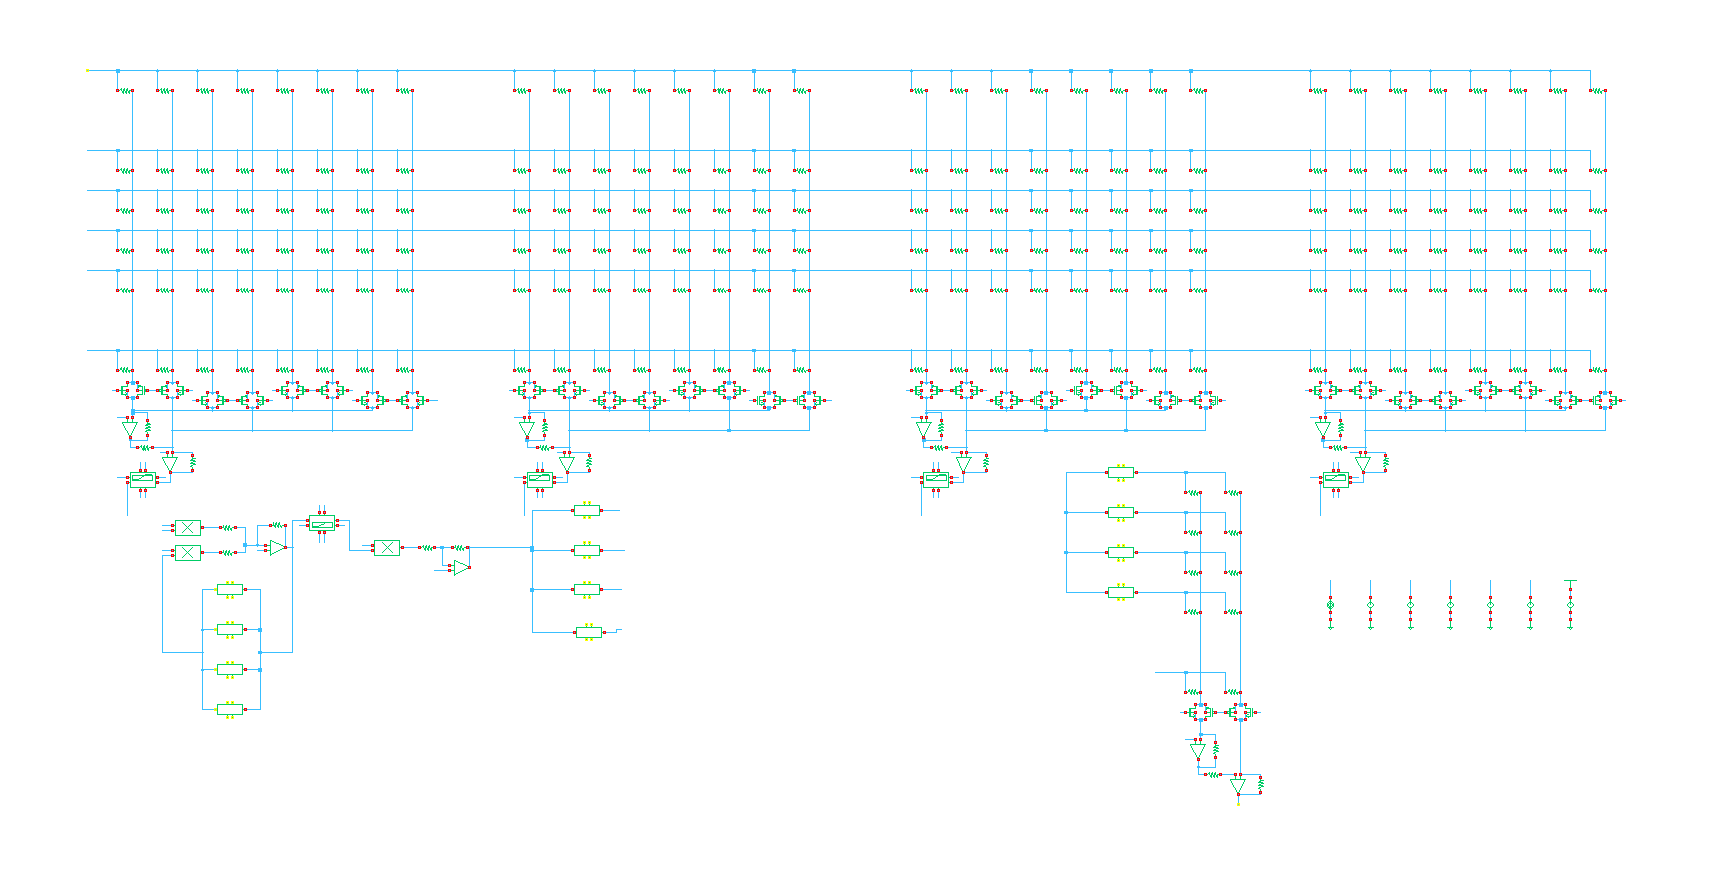
\includegraphics[width=\textwidth]{lstm/lstm-np}
  \end{frame}

  \begin{frame}
    \frametitle{Last weeks...}

    Last meeting, I promised to do :

    \centering
    \rowcolors{2}{evenRow}{oddRow}
    \begin{tabular}{c p{0.3\textwidth} c p{0.3\textwidth} c}
      \rowcolor{firstRow}
      \color{white}\textbf{\#} & \centering\color{white}Task & \color{white}Done? & \color{white}Why not? & \color{white}Help? \\
      0 & Work on thesis & onGoing & & No\\
      0.1 & Formula onChip Area & Almost & & No\\
      0.2 & power consumption & No & How would I approximate ? & Yes \\
      1 & Find another LSTM problem & Yes and no & Found one but too complicated & No\\
      1.1 & Mbedded Video stabilization & Yes & & No\\
      2 & Digital inference time & No & & No\\
    \end{tabular}

  \end{frame}

  \begin{frame}{What's new}
    \begin{itemize}
      \item Results obtianed :
        \begin{itemize}
            \color{text}
          \item
        \end{itemize}
      \item Improvements :
        \begin{itemize}
            \color{text}
          \item
        \end{itemize}
      \item Relevant information :
        \begin{itemize}
            \color{text}
          \item I started really focusing on the writing of the thesis. I'll have few to no updates from now on. (No idea what else to do)
        \end{itemize}
    \end{itemize}
  \end{frame}

  \begin{frame}
    \frametitle{Problems/doubts}
    I am wondering what goes in the :
    \begin{itemize}
      \item abstract
      \item thesis outline
    \end{itemize}
  \end{frame}

  \begin{frame}{Next weeks}

    List of what I plan to do in the next weeks :

    \centering
    \rowcolors{2}{evenRow}{oddRow}
    \begin{tabular}{ c m{6cm} }
      \rowcolor{firstRow}
      \color{white}\textbf{\#} & \centering\color{white}Task \cr
      0 & Work on thesis \\
      0.1 & Formula onChip Area \\
      0.2 & power consumption \\
      1 & Find another LSTM problem (optionnal) \\
      2 & Digital inference time \\
    \end{tabular}
  \end{frame}

  \begin{frame}{Networking and sharing}
    \begin{tikzpicture}
      \leftRect{Help/Collaboration :}{- If anybody has any idea of an interesting LSTM/NN problem to work on.}

      \rightRect{Recommendations :}{None}
    \end{tikzpicture}
  \end{frame}

\end{document}
